%
\hsection{Creating the Table}%
%
\begin{figure}%
\centering%
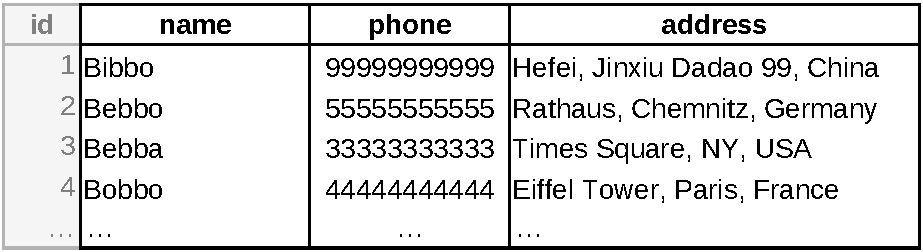
\includegraphics[width=0.72\linewidth]{\currentDir/dbStructureCustomer}%
\caption{How our table~\sqlil{customer} could look like if we designed it in a spreadsheet software like \microsoftExcel\ or \libreofficeCalc.}%
\label{fig:dbStructureCustomer}%
\end{figure}%
%
\gitLoadAndExecSQL{factory:create_table_customer}{}{factory}{create_table_customer.sql}{factory}{boss}{superboss123}%
\listingSQLandOutput{factory:create_table_customer}{%
Creating the table \textil{customer} to store the information about our factory's customers.%
}{}%
%
We will fittingly call the table for customers~\sqlil{customer}.
The structure of the table could look a bit like \cref{fig:dbStructureCustomer}~(if it was a \microsoftExcel\ or \libreofficeCalc\ spreadsheet):
For the minimalistic example here, it will be sufficient to store the name, mobile phone number, and address of the customers.%
%
\begin{sloppypar}%
We create the table \sqlil{customer} using the \sqlil{CREATE TABLE}\sqlIdx{CREATE!TABLE}\sqlIdx{TABLE} command in \cref{lst:factory:create_table_customer}.
The first column again should be the primary key~\sqlil{id}, which we again define as \sqlil{INT GENERATED BY DEFAULT AS IDENTITY PRIMARY KEY}\sqlIdx{INT}\sqlIdx{GENERATED}\sqlIdx{BY DEFAULT}\sqlIdx{PRIMARY KEY}\sqlIdx{IDENTITY}.
\end{sloppypar}%
%
Customers have names, so we again need a \sqlil{name} column.
Names can have different length, but 100~characters seems to be a reasonable limit.
Therefore, we will again use \sqlil{VARCHAR(100)}\sqlIdx{VARCHAR}.
For each customer, a name must be specified, so we again also write \sqlilIdx{NOT NULL}.
Do names need to be unique?
No they don't.
There can easily be two different customers with the same name.
Therefore, we will \emph{not} require this column to be \sqlilIdx{UNIQUE}.

However, when thinking about names, we realize that \sqlilIdx{NOT NULL} is not really a good bottom line for valid names.
If we enforce that names must always be entered {\dots} is that enough to ensure that names are \emph{correct}?
Actually, if we go back to our previous table \sqlil{product}, we find that we could easily enter a product with the name \sqlil{' bla     blab  '}, \sqlil{' '}, or even an empty name~\sqlil{''}.
We just demanded that the name be set, not that it cannot be set to a text string of length~0.

What does \emph{correct} actually mean?
If we enter \inQuotes{Bebbo} as customer name, clearly a \dbms\ cannot ensure that the real name of the person we mean is actually \inQuotes{Bebbo.}
Maybe that \inQuotes{Bebbo} person lied to our customer representative and intentionally gave a wrong name.
Maybe there was a misunderstanding and their name is actually \inQuotes{Beb-B\'o.}
No \dbms\ can guard against this.
But there are other sources of errors:
Maybe the person who types the name into our \dbms\ made an error!
Maybe they typed \inQuotes{ Bebbo}, i.e., accidentally hit space (the \keys{\space}~key) when beginning to write.
Such a tiny error could be invisible but could cause all sorts of issues down the line.
Or maybe they hit \keys{\tab} when entering the name, leaving an empty string in the form field.
These are the kind of errors that we want to prevent.
And we try to do this by specifying validity constraints at all levels of our application.

So what would be a good bottom line for valid names?
Well, it should probably start with a \inQuotes{word character}, say, \inQuotes{A}, \inQuotes{b}, or even~\inQuotes{张} and also end with one.
Inbetween, we would allow arbitrary characters.
This does not prevent anybody from entering \inQuotes{sgjw9345 s熊猫fki345Q} as name, but at least we would prevent the user from accidentally entering leading or trailing space characters or entering an empty name.
How can we accomplish that?%
%
\begin{sloppypar}%
\sql\ offers the mechanism of \emph{constraints}~\cite{PGDG:PD:C}.
Actually, \sqlilIdx{NOT NULL} and \sqlilIdx{UNIQUE} are shorthands for two constraints.
But we can also define more fancy ones.
Constraints can be written directly after declaring the columns in the \sqlil{CREATE TABLE}\sqlIdx{CREATE!TABLE}\sqlIdx{TABLE} command.
The syntax for this is \sqlil{CONSTRAINT constraint_name CHECK (expression)}\sqlIdx{CONSTRAINT!CHECK}.
In other words, we give the constraint a name and provide an expression that should be checked whenever data is entered or changed in the table.
Only if the expression is \sqlilIdx{TRUE} the insertion or change is permitted.%
\end{sloppypar}%
%
%
\sqlSyntax{syntax/create_table_constraint.sql}%
%
This means that we have to figure out how we can define \inQuotes{\sqlil{name} must start and end with a \inQuotes{word character} and can have arbitrary characters inbetween.} as such an expression.
This is a bit beyond what we can do with \sqlilIdx{LIKE}.
Luckily, \pglspl{regex} come to the rescue.
\Pglspl{regex} are text patterns that can be matched against text strings.
They are supported by many tools and programming languages~(such as \python~\cite{programmingWithPython}), and also by \sql\ and, hence, \postgresql~\cite{PGDG:PD:PRE}.
\Pglspl{regex} are a whole different kind of subject that you can read about in~\cite{PGDG:PD:PRE}.
Here we will just briefly introduce and directly use them.

We will define the constraint that the values in the column~\sqlil{name} must match to the \pgls{regex} \sqlil{'^\\w.*\\w\$'}.
The \textil{^}~matches the beginning of a text.
\textil{\\w}~stands for a single \inQuotes{word character},
\textil{^\\w}~thus means that the text string must start with a word character.
\textil{.}~passt auf jedes beliebige Zeichen.
\textil{*}~means that the expression item directly before the \textil{*} can occur any number of times, from zero to infinity.
Hence, the \textil{.*} following the \textil{^\\w} means that, after the word character at the beginning of the text, an arbitrary number of arbitrary characters may follow.
Finally, \textil{\$}~matches to the end of the text.
Therefore, the~\textil{\\w\$}~at the end of the \pgls{regex} means that the text that we compare the \pgls{regex} with must have a word character at its end for the \pgls{regex} to match.

In summary, by writing \sqlil{'^\\w.*\\w\$'}, we say:
The beginning of the text, i.e., the very first character, must be a \inQuotes{word character}, e.g., \inQuotes{A}, \inQuotes{b}, or \inQuotes{李}.
Then, there can be an arbitrary number of other characters, including spaces, numbers, signs, whatever.
At the end of the text, we again expect a word character.
This means that we demand that names consist of at least two word characters.
We could refine this to also allow single-character names, to prevent characters such as \inQuotes{@} from occurring, etc., but let's keep it at this for now.%
%
\begin{sloppypar}%
Having a reasonable limitation for the name, we now define the rule \sqlil{customer_name_ok} as \sqlil{CONSTRAINT customer_name_ok CHECK (name \~ '^\\w.*\\w\$')}\sqlIdx{{\textbackslash}w}\sqlIdx{\$}\sqlIdx{\textasciicircum}\sqlIdx{.}\sqlIdx{\textasciitilde}.
The \sqlilIdx{CONSTRAINT} marks the beginning of a constraint, \sqlil{customer_name_ok} is the name, and \sqlilIdx{CHECK}\sqlIdx{CONSTRAINT!CHECK} tell us that we will next define an expression~(as opposed to simply \sqlilIdx{NOT NULL}).
\sqlil{(name \~ '^\\w.*\\w\$')}\sqlIdx{{\textbackslash}w}\sqlIdx{\$}\sqlIdx{\textasciicircum}\sqlIdx{.}\sqlIdx{\textasciitilde} says that the field \sqlil{name} must match the \pgls{regex} \sqlil{'^\\w.*\\w\$'}.
Here, \sqlil{\~}\sqlIdx{\textasciitilde} stands for \pgls{regex}-based pattern matching.
With this, the names \inQuotes{S} and \inQuotes{  schwipschawp } are prohibited, but \inQuotes{Thomas Weise} and \inQuotes{熊猫先生} are OK.%
\end{sloppypar}%
%
Each customer also needs to have a phone number, so we add a column~\sqlil{phone}.
While phone numbers may appear to be integer numbers, they could have leading zeros.
Therefore, we will store them as text strings.
In China, landlines have 10~digits and mobile numbers have 11~digits~\cite{BD2006BDBK:MPNANSBTTMDFMP}.
Therefore, we choose~\sqlil{VARCHAR(11)}\sqlIdx{VARCHAR} as the datatype.
The phone numbers must be~\sqlilIdx{NOT NULL} and this time, we also insist on them to be~\sqlilIdx{UNIQUE}.
While there might be two different customers with the same name, we do not permit two different customers having the same phone number.
Indeed, if our sales department wants to enter a customer's information into the \db\ and there is already one record with the same phone number, then most likely this would be the same customer and they are in the process of creating a duplicate entry by accident.

Now we want to limit the phone number text to represent valid phone numbers.
\sqlil{'ABC'}, for example, is not a valid phone number and neither is~\sqlil{1}.
We want to only permit numbers consisting of ten to eleven digits.
We can do this in exactly the same way in which guarded our \sqlil{name} field:
by defining a constraint.
We write \sqlil{CONSTRAINT customer_phone_ok CHECK (phone ~ '^\\d\{10,11\}\$')}\sqlIdx{CONSTRAINT!CHECK}\sqlIdx{{\textbackslash}d}\sqlIdx{\$}\sqlIdx{\textasciicircum}\sqlIdx{\textasciitilde}.
The name of the constraint will be \sqlil{customer_phone_ok}.
We again match a \pgls{regex} via \sqlIdx{\textasciitilde}\sqlil{\~}, but this time we match the value of~\sqlil{phone}.

The \pgls{regex} \sqlil{'\^\\d\{10,11\}\$'}\sqlIdx{{\textbackslash}d}\sqlIdx{\$}\sqlIdx{\textasciicircum} reads as follows:
At the start of the text~(denoted by~\textil{\^}\sqlIdx{\textasciicircum}), there is a sequence of 10 to~11 digits, and then comes the end of the text~(denoted by~\textil{\$}\sqlIdx{\$}).
Here, \textil{\\d}\sqlIdx{{\textbackslash}d}\ stands for a single character that is a digit, i.e.,~0\dots9.
The \textil{\{10,11\}} specfies between 10 and 11 repetitions of this pattern.
Therefore, our constraint requires that any value of \sqlil{phone} to be stored consists of ten to eleven digits~(and only digits).
This rules out phone numbers containing other characters, as well as customers registering under number~110.

Of course, this still does not guarantee that the phone numbers that are entered are valid.
On the one hand, we could have a much more complex expression that checks whether the ten-digit numbers have proper area codes as their first digits and that the eleven-digit numbers start with proper mobile phone provider prefixes.
On the other hand, there still would be no way to verify, from within \sql\ at least, that the phone number actually exists.
Then again, even if we could check that, we still would not know whether the phone number is registered under the customer's name.
These things are far beyond the scope here.
To keep the \db\ clean, the simple check defined here shall suffice.

Finally, each customer should have a shipping address.
Here we will just settle for \sqlil{VARCHAR(255)}.
A length of at most 255~characters seems reasonable, as 255~is also used in many other systems as the limit.
We require the \sqlil{address} to be \sqlilIdx{NOT NULL}, but it does \emph{not} have to be \sqlilIdx{UNIQUE}.
For laziness sake I will not specify a \sqlilIdx{CONSTRAINT} that sanity-checks addresses {\dots} maybe you could do this as a small exercise when reproducing the example?

Either way, the full \sql\ command for creating our table \sqlil{customer} is given in \cref{lst:factory:create_table_customer}.
Notice that we, again, use the \textil{boss} user with password \textil{superboss123} to execute these commands.
We create the table and, afterwards, check whether a new table appeared in the \sqlilIdx{pg\_catalog.pg\_tables}.
It does: the user \textil{boss} now owns two tables, \sqlil{product} and \sqlil{customer}, as you can see in \cref{exec:factory:create_table_customer}.%
%
\endhsection%
%
